\documentclass[aspectratio=169, table]{beamer}

\usepackage{colortbl}
\usepackage{xcolor}
\usepackage{listings}
\usepackage{tikz}
\usepackage{pgfplots}
\usepgfplotslibrary{polar}
\usetikzlibrary{arrows.meta, positioning, calc}

\usetheme{Pradita}


\usepackage{listings}
\lstdefinestyle{SqlStyle}{
language=SQL,
basicstyle=\ttfamily\footnotesize,
morekeywords={REAL, TEXT, REFERENCES},
keywordstyle=\color{blue},
commentstyle=\color{gray},
stringstyle=\color{red},
breaklines=true,
showstringspaces=false,
tabsize=2,
captionpos=b,
numbers=left,
numberstyle=\tiny\color{gray},
frame=lines,
backgroundcolor=\color{lightgray!10},
comment=[l]{//},
morecomment=[s]{/*}{*/},
commentstyle=\color{gray}\ttfamily,
string=[s]{'}{'},
morestring=[s]{"}{"},
%	stringstyle=\color{teal}\ttfamily,
%	showstringspaces=false
}

\lstdefinelanguage{bash} {
keywords={},
basicstyle=\ttfamily\small,
keywordstyle=\color{blue}\bfseries,
ndkeywords={iex},
ndkeywordstyle=\color{purple}\bfseries,
sensitive=true,
commentstyle=\color{gray},
stringstyle=\color{red},
numbers=left,
numberstyle=\tiny\color{gray},
breaklines=true,
frame=lines,
backgroundcolor=\color{lightgray!10},
tabsize=2,
comment=[l]{\#},
morecomment=[s]{/*}{*/},
commentstyle=\color{gray}\ttfamily,
stringstyle=\color{purple}\ttfamily,
showstringspaces=false
}

% Define Java language style for listings
\lstdefinestyle{JavaScript}{
	language=Java,
	basicstyle=\ttfamily\footnotesize,
	keywordstyle=\color{blue},
	commentstyle=\color{gray},
	stringstyle=\color{red},
	breaklines=true,
	showstringspaces=false,
	tabsize=4,
	captionpos=b,
	numbers=left,
	numberstyle=\tiny\color{gray},
	frame=lines,
	backgroundcolor=\color{lightgray!10},
	comment=[l]{//},
	morecomment=[s]{/*}{*/},
	commentstyle=\color{gray}\ttfamily,
	string=[s]{'}{'},
	morestring=[s]{"}{"},
	%	stringstyle=\color{teal}\ttfamily,
	%	showstringspaces=false
}

\title{\Huge Intro to Supervised \\
\vspace{10pt}
Machine Learning}
\subtitle{IT140704 - Big Data for Business}
%\date[Serial]{Penggunaan Large Language Model untuk Pengajaran}
\author{\textbf{Alfa Yohannis}}
\begin{document}

\frame{\titlepage}


\begin{frame}[fragile]
\frametitle{Contents}
\vspace{20pt}
\begin{columns}[t]
	\column{0.5\textwidth}
	\tableofcontents[sections={1-5}]
	
	\column{0.5\textwidth}
	\tableofcontents[sections={6-20}]
\end{columns}
\end{frame}

\begin{frame}{\hfill}
	\centering
	\Huge{\textbf{How can data be used to create real strategic, tactical, and operational values?}}
\end{frame}


\section{Role of Machine Learning in the Big Data Era}

\begin{frame}{Role of Machine Learning in the Big Data Era}
	\vspace{20pt}
	\begin{itemize}
		\item \textbf{Big Data Landscape.} Defined by volume, velocity, variety, veracity, and value, requiring advanced analytics.
		\item \textbf{ML's Strategic Role.} Critical in the value chain for analysing and extracting insights from large datasets.
		\item \textbf{Beyond Description.} Enables predictive and prescriptive analytics for smarter, faster decisions.
		\item \textbf{Real-World Applications.} Used for churn prediction, fraud detection, demand forecasting, and recommendations.
		\item \textbf{Empowering Leaders.} Understanding supervised learning helps non-technical managers work effectively with data teams.
	\end{itemize}
\end{frame}

\section{Types of Learning in Machine Learning}

\begin{frame}{Types of Learning in Machine Learning}
	\vspace{20pt}
	\begin{itemize}
		\item \textbf{Supervised Learning.} Learns from labelled data to predict future outcomes. Common in business for churn prediction, credit scoring, and sales forecasting. Easy to evaluate and widely used due to available historical data.
		
		\item \textbf{Unsupervised Learning.} Finds hidden patterns in unlabelled data. Useful for customer segmentation and anomaly detection using clustering or dimensionality reduction techniques.
		
		\item \textbf{Reinforcement Learning.} Agent learns by interacting with its environment, receiving rewards or penalties. Used in dynamic pricing and ad placement.
		
		\item \textbf{Business Focus.} Supervised learning is the most practical for business due to clear labels and measurable impact on decisions.
	\end{itemize}
\end{frame}

\section{Basic Concept of Supervised Learning}

\begin{frame}{Basic Concept of Supervised Learning}
	\vspace{20pt}
	\begin{itemize}
		\item \textbf{Definition.} Supervised learning maps input features (\textbf{X}) to output labels (\textbf{Y}) using labelled data.
		\item \textbf{Business Example.} For churn prediction:
		\begin{itemize}
			\item \textit{Features (X):} call frequency, recent usage, payment status, subscription length.
			\item \textit{Label (Y):} \texttt{1} for churn, \texttt{0} otherwise.
		\end{itemize}
		\item \textbf{Classification.} Predicts discrete labels (e.g., churn yes/no, fraud or not). Common algorithms: Decision Tree, Logistic Regression, SVM.
		\item \textbf{Regression.} Predicts continuous values (e.g., sales, revenue). Common algorithms: Linear Regression, Lasso, Gradient Boosting.
		\item \textbf{Why It Matters.} Enables proactive, data-driven decisions for reducing risk and improving efficiency.
	\end{itemize}
\end{frame}

\section{Popular Algorithms for Supervised Learning}

\begin{frame}{Linear Regression}
	\vspace{10pt}
	\begin{columns}
		\column{0.5\textwidth}
		\begin{itemize}
			\item \textbf{Linear Regression} is a predictive algorithm used to estimate continuous values such as sales, revenue, or product demand.
			\item It works by finding the best-fitting straight line that represents the relationship between features (e.g., number of ads) and the label (e.g., total sales).
			\item \textbf{Business Use Case:} Estimating how digital promotion frequency affects overall sales.
		\end{itemize}
		
		\column{0.5\textwidth}
		\begin{figure}
			\centering
			\begin{tikzpicture}[scale=1]
				% Axis
				\draw[->] (0,0) -- (6.5,0) node[below left] {\scriptsize Promotions};
				\draw[->] (0,0) -- (0,5) node[above left] {\scriptsize Sales};
				
				% Sample data points
				\filldraw[blue] (0.5,1.2) circle (2pt);
				\filldraw[blue] (1.5,1.6) circle (2pt);
				\filldraw[blue] (2.0,2.1) circle (2pt);
				\filldraw[blue] (3.0,2.7) circle (2pt);
				\filldraw[blue] (4.0,3.5) circle (2pt);
				\filldraw[blue] (5.5,4.2) circle (2pt);
				
				% Regression line
				\draw[thick, red] (0.3,1) -- (6,4.5);
				\node[red] at (4.2,4.3) {\tiny Trend Line};
				
				% Optional grid
				\foreach \x in {1,2,3,4,5} {
					\draw[dashed, gray!50] (\x,0) -- (\x,4.8);
				}
			\end{tikzpicture}
		\end{figure}
	\end{columns}
\end{frame}

\begin{frame}{Logistic Regression}
	\vspace{10pt}
	\begin{columns}
		\column{0.45\textwidth}
		\begin{itemize}
			\item \textbf{Logistic Regression} is used for binary classification—predicting outcomes like \textit{Yes/No}, \textit{Churn/Not}, or \textit{Pass/Fail}.
			\item It estimates the probability of an outcome and applies a threshold (e.g., 0.5) to assign a class.
			\item \textbf{Business Example:} Predicting whether a customer will churn based on interaction history.
		\end{itemize}
		
		\column{0.55\textwidth}
		\begin{figure}
			\centering
			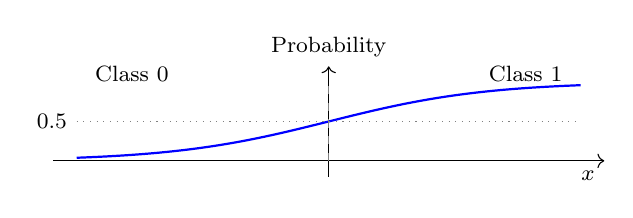
\begin{tikzpicture}[scale=1]
				% Axis
				\draw[->] (-3.5,0) -- (3.5,0) node[below left] {\footnotesize $x$};
				\draw[->] (0,-0.2) -- (0,1.2) node[above] {\footnotesize Probability};
				
				% Sigmoid curve
				\draw[thick, domain=-3.2:3.2, samples=100, smooth, variable=\x, blue]
				plot ({\x}, {1/(1 + exp(-\x))});
				
				% Dotted line at x=0
				\draw[dashed, gray] (0,0) -- (0,1);
				
				% Threshold line
				\draw[dotted, gray] (-3.2,0.5) -- (3.2,0.5);
				\node[left] at (-3.2,0.5) {\footnotesize 0.5};
				
				% Class labels
				\node at (-2.5,1.1) {\footnotesize Class 0};
				\node at (2.5,1.1) {\footnotesize Class 1};
			\end{tikzpicture}
		\end{figure}
	\end{columns}
\end{frame}

\begin{frame}{Decision Tree}
	\vspace{10pt}
	\begin{columns}
		\column{0.49\textwidth}
		\begin{itemize}
			\item \textbf{Decision Tree} mimics human decision-making using “if–then” logic represented in a tree structure.
			\item Each branch represents a condition based on input features; each leaf gives a final prediction.
			\item \textbf{Business Example:} Evaluating loan eligibility based on income, age, home ownership, and credit history.
			\item Its main strength is transparency—business users can easily trace and interpret the prediction path.
		\end{itemize}
		
		\column{0.51\textwidth}
		\begin{figure}
			\centering
			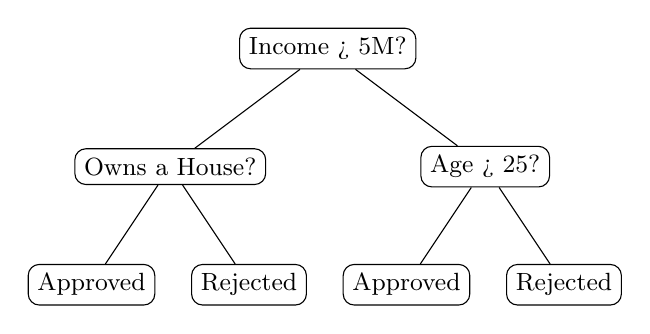
\begin{tikzpicture}[
				level 1/.style={sibling distance=40mm},
				level 2/.style={sibling distance=20mm},
				level distance=15mm,
				every node/.style={draw, rectangle, rounded corners, align=center, font=\small}
				]
				\node {Income > 5M?}
				child {node {Owns a House?}
					child {node {Approved}}
					child {node {Rejected}}
				}
				child {node {Age > 25?}
					child {node {Approved}}
					child {node {Rejected}}
				};
			\end{tikzpicture}
		\end{figure}
	\end{columns}
\end{frame}

\begin{frame}{K-Nearest Neighbours (K-NN)}
	\vspace{10pt}
	\begin{columns}
		\column{0.45\textwidth}
		\begin{itemize}
			\item \textbf{K-Nearest Neighbours (K-NN)} compares new data to historical data points based on distance similarity.
			\item The model stores all training data and classifies new input by majority vote from its closest neighbours.
			\item \textbf{Business Example:} Classifying a new customer by identifying and following the dominant class of similar past customers.
		\end{itemize}
		
		\column{0.55\textwidth}
		\begin{figure}
			\centering
			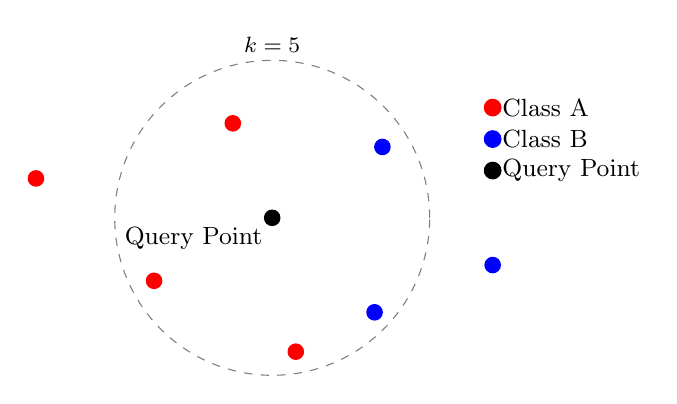
\begin{tikzpicture}[scale=1, every node/.style={font=\small}]
				
				% Query point
				\fill[black] (0,0) circle (3pt);
				\node[below left] at (0,0) {Query Point};
				
				% Neighbourhood radius
				\draw[gray, dashed] (0,0) circle (2);
				
				% Red class points
				\fill[red] (-0.5, 1.2) circle (3pt);
				\fill[red] (-1.5, -0.8) circle (3pt);
				\fill[red] (0.3, -1.7) circle (3pt);
				
				% Blue class points
				\fill[blue] (1.4, 0.9) circle (3pt);
				\fill[blue] (1.3, -1.2) circle (3pt);
				
				% Outside radius
				\fill[red] (-3, 0.5) circle (3pt);
				\fill[blue] (2.8, -0.6) circle (3pt);
				
				% Legend
				\draw[red, fill=red] (2.8,1.4) circle (3pt);
				\node[right] at (2.8,1.4) {Class A};
				
				\draw[blue, fill=blue] (2.8,1.0) circle (3pt);
				\node[right] at (2.8,1.0) {Class B};
				
				\draw[black, fill=black] (2.8,0.6) circle (3pt);
				\node[right] at (2.8,0.6) {Query Point};
				
				% Label k
				\node at (0,2.2) {\footnotesize $k = 5$};
				
			\end{tikzpicture}
		\end{figure}
	\end{columns}
\end{frame}

\section{Stages of a Machine Learning Project in Big Data}

\begin{frame}{ML Project Lifecycle in Big Data Context}
	\vspace{10pt}
	\begin{itemize}
		\item \textbf{1. Data Collection.} Collect high-volume, diverse data from CRM, ERP, IoT, or social media using tools like Kafka or Hadoop.
		\item \textbf{2. Data Preparation.} Clean, transform, and select relevant features. Automate for scalability.
		\item \textbf{3. Algorithm Selection.} Choose based on task type and interpretability—e.g., Decision Tree or Gradient Boosting.
		\item \textbf{4. Model Training.} Train using distributed platforms like Spark or TensorFlow.
		\item \textbf{5. Evaluation.} Use metrics like accuracy or RMSE and assess business value.
		\item \textbf{6. Interpretation.} Ensure results are understandable, actionable, and aligned with business goals.
	\end{itemize}
\end{frame}



\section{Practical Steps with Orange}

\begin{frame}{Steps to Build a Decision Tree with Orange}
	\vspace{10pt}
	\begin{itemize}
		\item \textbf{Install Orange:} Download from \url{https://orangedatamining.com} and install for your OS.
		
		\item \textbf{Prepare Dataset:} Use \texttt{loan.csv} from \url{https://u.pcloud.link/publink/show?code=kZnR3B5Z8TazEXoFXx7LJ4K87WksvXM0gu1X} with fields like income, credit score, and loan approval.
		
		\item \textbf{Build Workflow:} Add \texttt{File}, \texttt{Data Table}, \texttt{Select Columns}, \texttt{Tree}, \texttt{Tree Viewer}, \texttt{Test \& Score}, and \texttt{Confusion Matrix} components.
		
		\item \textbf{Interpret Results:} Analyse decision paths and model metrics to understand key features behind loan approval predictions.
	\end{itemize}
\end{frame}


\begin{frame}{Orange Workflow for Loan Approval Model}
	\vspace{10pt}
	\centering
	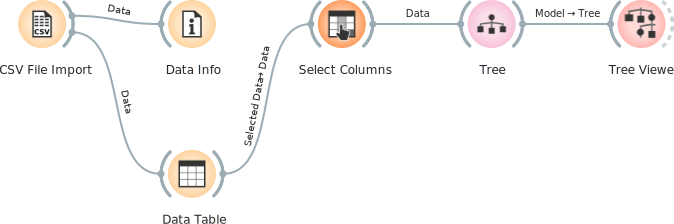
\includegraphics[width=\linewidth]{../../figures/decision_tree_pipeline.png}
\end{frame}


\begin{frame}{Building a Decision Tree from Loan Data}
	\vspace{10pt}
	After loading \texttt{loan.csv} and setting \texttt{loan\_approved} as the target, students use Orange’s \texttt{Tree} component to build a transparent, easy-to-understand model suitable for managerial analysis.
	
	\begin{itemize}
		\item \textbf{Splitting Criteria:} Orange selects attributes using \textit{Information Gain} or \textit{Gini Index}.
		\item \textbf{Tree Construction:} Data is recursively split until a maximum depth or stopping condition is met.
		\item \textbf{Overfitting Control:} Limit depth, set minimum samples, and apply pruning options for balance.
	\end{itemize}
	
	Students are encouraged to compare tree depths, examine root and leaf nodes, and interpret decision paths for credit approval strategy.
\end{frame}


\begin{frame}{Visualisation, Interpretation, Business Insight}
	\vspace{10pt}
	Decision trees are highly interpretable and visually accessible. In Orange, the \texttt{Tree Viewer} displays the decision path using conditions like:
	\begin{itemize}
		\item \texttt{credit\_score = Good}
		\item \texttt{has\_collateral = True}
		\item \texttt{income\_level = Medium}
	\end{itemize}
	
	Leaf nodes show predictions (\texttt{Yes}/\texttt{No}), sample counts, and class ratios.
	
	Students can explore:
	\begin{itemize}
		\item Which profiles are most likely to get loan approval?
		\item What features drive credit decisions?
		\item How can the model guide segment-based lending strategies?
	\end{itemize}
	
	This supports fact-based credit policy, what-if exploration, and clearer communication across business units.
\end{frame}

\begin{frame}{Decision Tree Output from \texttt{loan.csv}}
	\vspace{20pt}
	\centering
	\includegraphics[width=.9\linewidth]{../../figures/loan_tree.png}
\end{frame}

\begin{frame}{What-If Scenarios \& Customer Segmentation}
	\vspace{10pt}
	Decision trees support “what-if” analysis by allowing users to simulate changes in attributes and observe how predictions shift. In Orange, students can interactively modify values (e.g., \texttt{credit\_score}, \texttt{employment\_status}) and trace changes in approval decisions.
	
	\textbf{Example:}
	From \texttt{Unemployed}, \texttt{Bad}, \texttt{No Collateral} → \texttt{Denied},  
	to \texttt{Employed}, \texttt{Good}, \texttt{Has Collateral} → \texttt{Approved}.
	
	Each decision path represents a customer segment. These can be used to:
	\begin{itemize}
		\item Tailor credit policies by segment.
		\item Adjust interest terms by profile.
		\item Prioritise applications by approval likelihood.
	\end{itemize}
	
	Trees empower precise, evidence-based segmentation and strategy.
\end{frame}

\section{Model Evaluation and Performance Metrics}

\begin{frame}{Model Evaluation and Performance Metrics}
	\vspace{10pt}
	Evaluating a supervised learning model ensures that predictions are both accurate and business-relevant. In loan approval scenarios, Orange’s \texttt{Test \& Score} component provides intuitive metrics:
	
	\begin{itemize}
		\item \textbf{Accuracy:} Proportion of correct predictions. Simple to understand but misleading if classes are imbalanced.
		\item \textbf{Precision:} Among predicted approvals, how many were truly approved. High precision reduces risky approvals.
		\item \textbf{Recall:} Among actual approved cases, how many were correctly predicted. Important to avoid missing good applicants.
		\item \textbf{F1-Score:} Harmonic mean of precision and recall—used when both false positives and false negatives matter.
	\end{itemize}
	
	These metrics guide business strategies for balancing risk and opportunity.
\end{frame}

\begin{frame}{Choosing the Right Metrics}
	\vspace{10pt}
	No single metric fits all scenarios. Metric selection should align with business strategy:
	
	\begin{itemize}
		\item \textbf{If credit default risk is critical}, prioritise precision to avoid approving high-risk borrowers.
		\item \textbf{If financial inclusion is the goal}, focus on recall to avoid rejecting eligible applicants.
		\item \textbf{If both risks must be balanced}, use F1-score for a more proportional assessment.
	\end{itemize}
	
	Orange’s visual, code-free tools enable intuitive, iterative model assessment aligned with strategic decision-making.
\end{frame}

\section{Hands-On Model Evaluation}

\begin{frame}{Test and Score Results in Orange}
	\vspace{20pt}
	\centering
	\includegraphics[width=0.7\linewidth]{../../figures/decision_tree_results.png}
	
	The model’s performance across folds on accuracy, precision, recall, and F1-score.
\end{frame}


\begin{frame}{Evaluating Decision Tree Model in Orange}
	\vspace{5pt}
	Evaluation was conducted using the \textit{Orange} platform to assess the performance of a Decision Tree model on a classification dataset via the \texttt{Test and Score} widget:
	
	\begin{itemize}
		\item \textbf{Evaluation Method:} Cross Validation
		\item \textbf{Number of Folds:} 3 (3-Fold CV)
		\item \textbf{Stratified:} Enabled
		\item \textbf{Model:} Decision Tree
	\end{itemize}
	
	\textbf{Cross Validation} divides the dataset into multiple folds to iteratively train and test the model.\\
	  
	\textbf{Stratified CV} preserves class distribution within each fold, making it suitable for imbalanced classification problems.
\end{frame}


\begin{frame}{Evaluation Results and Interpretation}
	\vspace{5pt}
	\begin{columns}
		\column[t]{0.28\textwidth}
		
		\textbf{Evaluation Metrics:}
		\arrayrulecolor{black} % ensure black borders
		\begin{center}
			\begin{tabular}{|l|c|}
				\hline
				\textbf{Metric} & \textbf{Value} \\
				\hline
				AUC & 0.567 \\
				Accuracy & 0.500 \\
				F1 Score & 0.508 \\
				Precision & 0.521 \\
				Recall & 0.500 \\
				MCC & -0.043 \\
				\hline
			\end{tabular}
		\end{center}
		
		\column[t]{0.72\textwidth}
		\begin{itemize}
			\item \textbf{AUC 0.567 (Area Under Curve):} Slightly better than random; poor class separation.
			\item \textbf{Accuracy 0.500:} Model predicts correctly only half of the time.
			\item \textbf{F1 Score 0.508:} Indicates balanced but weak prediction strength.
			\item \textbf{Precision 0.521:} About half of predicted positives are correct.
			\item \textbf{Recall 0.500:} Model captures only half of actual positives.
			\item \textbf{MCC –0.043 (Matthews Correlation Coefficient):} Very low correlation between predictions and ground truth.
		\end{itemize}
	\end{columns}
\end{frame}


\begin{frame}{Preliminary Conclusion}
	\vspace{5pt}
	\subsection*{Preliminary Conclusion}
	
	Although the evaluation results are slightly better than before, the performance of the Decision Tree model remains low. An AUC slightly above 0.5 indicates the model is not yet optimal in distinguishing between classes. Possible reasons include:
	
	\begin{enumerate}
		\item \textbf{High data complexity} or weak patterns between features that the Decision Tree cannot easily learn.
		\item \textbf{Limited dataset size} leading to poor generalisation by the model.
		\item \textbf{Uninformative feature distribution} with respect to the target variable.
	\end{enumerate}
\end{frame}

\section{Confusion Matrix Analysis}

\subsection*{Visualisation and Explanation}

\begin{frame}{Confusion Matrix Analysis}
	\vspace{5pt}
	\begin{figure}
		\centering
		\includegraphics[width=0.7\linewidth]{../../figures/decision_tree_confusion_matrix.png}
	\end{figure}
	
	\vspace{-20pt}
	The confusion matrix is used to evaluate classification performance by comparing the number of correct and incorrect predictions for each class.
\end{frame}

\subsection*{Matrix Contents and Interpretation}

\begin{frame}{Matrix Contents and Interpretation}
	\vspace{5pt}
	\textbf{Matrix Contents:}
	\begin{center}
		\begin{tabular}{|c|c|c|c|}
			\hline
			& \textbf{Predicted: no} & \textbf{Predicted: yes} & \textbf{Total (Actual)} \\
			\hline
			\textbf{Actual: no} & 2 (True Negative) & 3 (False Positive) & 5 \\
			\textbf{Actual: yes} & 4 (False Negative) & 5 (True Positive) & 9 \\
			\hline
			\textbf{Total (Predicted)} & 6 & 8 & 14 \\
			\hline
		\end{tabular}
	\end{center}
	
	\vspace{8pt}
	\textbf{Interpretation:}
	\begin{itemize}
		\item \textbf{True Positive (TP):} 5 — Cases labeled \texttt{yes} correctly predicted as \texttt{yes}.
		\item \textbf{True Negative (TN):} 2 — Cases labeled \texttt{no} correctly predicted as \texttt{no}.
		\item \textbf{False Positive (FP):} 3 — Cases labeled \texttt{no} incorrectly predicted as \texttt{yes}.
		\item \textbf{False Negative (FN):} 4 — Cases labeled \texttt{yes} incorrectly predicted as \texttt{no}.
	\end{itemize}
\end{frame}

\subsection*{Metric Calculation and Conclusion}

\begin{frame}{Metric Calculation and Conclusion}
	\vspace{20pt}
	\begin{columns}
		\column[t]{0.45\textwidth}
		\textbf{Metric Calculation:}
		\vspace{5pt}
		\begin{itemize}
			\item \textbf{Accuracy} = \( \frac{TP + TN}{TP + TN + FP + FN} = \frac{5 + 2}{14} = 0.500 \)
			\item \textbf{Precision} = \( \frac{TP}{TP + FP} = \frac{5}{5 + 3} = 0.625 \)
			\item \textbf{Recall} = \( \frac{TP}{TP + FN} = \frac{5}{5 + 4} = 0.556 \)
			\item \textbf{F1 Score} = \( 2 \times \frac{0.625 \times 0.556}{0.625 + 0.556} \approx 0.588 \)
		\end{itemize}
		
		\column[t]{0.55\textwidth}
		\textbf{Note:} These metrics are calculated from the overall prediction aggregation, not from per-fold averages as in the \textit{Test and Score} component.
		
		\vspace{5pt}
		\textbf{Conclusion:}
		
		The Decision Tree model still shows moderate performance. From the confusion matrix, the model frequently misclassifies \texttt{yes} as \texttt{no} (FN = 4) and also produces several errors predicting \texttt{no} as \texttt{yes} (FP = 3).
		
		To improve accuracy, further exploration of alternative models, parameter tuning, and feature selection is recommended.
	\end{columns}
\end{frame}

\section{Summary}

\begin{frame}{Summary}
	\vspace{20pt}
	\begin{itemize}
		\item \textbf{Strategic Role:} Machine Learning enhances Big Data by enabling predictive and prescriptive analytics that support faster and smarter business decisions.
		\item \textbf{Business Applications:} Supervised learning is widely used in churn prediction, credit scoring, demand forecasting, and fraud detection.
		\item \textbf{Practical Tools:} Tools like Orange allow non-technical users to build and interpret decision tree models visually and intuitively.
		\item \textbf{Model Evaluation:} Key metrics such as accuracy, precision, recall, and F1-score help assess performance and business impact.
		\item \textbf{Decision Support:} Transparent models like decision trees make it easier for managers to justify and communicate data-driven decisions.
	\end{itemize}
\end{frame}


\end{document}
